\section{Estudio de Rendimiento}

Para el estudio de rendimiento de utilizo la cantidad de tiempo entre rutinas relevantes a cada prueba en milisegundos. Para obtener tiempos precisos en GPU se utilizó el software GPU PerfStudio y análisis de frame. Este software nos permite observar los detalles en el pipeline de renderizado y tiempo total de cada llamada de dibujo o \emph{draw call} al API grafico OpenGL

\subsection{Prueba Base}
La prueba base de rendimiento comprende todos los pasos del algoritmo sin trazado de sombras o modificaciones sobre la escena estática. Para esta prueba se colocó la aplicación en actualización forzosa de tal manera que todos los pasos del algoritmo se realicen por frame. También se varían tres aspectos de la aplicación: resolución de pantalla, dimensión de la representación en vóxeles y factor de longitud de marcha del cono.

Estas pruebas utilizan todas las escenas completas. La configuración del escenario comprende una luz direccional con mapeado de sombras, y tres modelos precargados. Los modelos utilizados son Stanford Happy Buddha, Stanford Dragon y Stanford Bunny, estos modelos fueron seleccionados por su complejidad geométrica. Cada modelo tiene su propio material con un cono especular de apertura 45, 27 y 9 grados respectivamente. La cámara en escena es colocada de tal forma que todos los fragmentos visibles formen parte del trazado de conos. 

\begin{table}[h]
\centering
\begin{tabular}{llllllllll}
\rot{Escena}                    & \rot{Voxelización Estática} & \rot{Limpieza de Vóxeles Dinámicos} & \rot{Voxelización Dinámica} & \rot{Sombreado de Vóxeles} & \rot{Mipmapping Direccional} & \rot{Iluminación Global de Vóxeles} & \rot{Mipmapping Direccional} & \rot{Trazado de Conos con Vóxeles} & \rot{Tiempo Dinámico}    \\ \hline
\multicolumn{1}{|l|}{Sibenik}     & \multicolumn{1}{l|}{1.80}     & 0.58                                  & \multicolumn{1}{l|}{2.11}     & 0.95                         & \multicolumn{1}{l|}{1.39}      & 3.88                                  & \multicolumn{1}{l|}{1.38}      & \multicolumn{1}{l|}{7.31}            & \multicolumn{1}{l|}{17.60} \\
\multicolumn{1}{|l|}{Cornell Box} & \multicolumn{1}{l|}{0.51}     & 0.78                                  & \multicolumn{1}{l|}{1.30}     & 1.33                         & \multicolumn{1}{l|}{1.38}      & 8.41                                  & \multicolumn{1}{l|}{1.37}      & \multicolumn{1}{l|}{7.23}            & \multicolumn{1}{l|}{21.81} \\
\multicolumn{1}{|l|}{Conference}  & \multicolumn{1}{l|}{46.04}    & 0.56                                  & \multicolumn{1}{l|}{1.52}     & 0.86                         & \multicolumn{1}{l|}{1.38}      & 3.23                                  & \multicolumn{1}{l|}{1.37}      & \multicolumn{1}{l|}{7.50}            & \multicolumn{1}{l|}{16.42} \\
\multicolumn{1}{|l|}{Sponza}      & \multicolumn{1}{l|}{11.29}    & 0.60                                  & \multicolumn{1}{l|}{2.03}     & 1.13                         & \multicolumn{1}{l|}{1.37}      & 5.44                                  & \multicolumn{1}{l|}{1.38}      & \multicolumn{1}{l|}{7.01}            & \multicolumn{1}{l|}{18.97} \\ \hline
\end{tabular}
\captionsetup{justification=centering}
\caption{Rendimiento de todas las partes del algoritmo en distintas escenas utilizando volumenes de resolución $256^3$, factor de longitud de marcha de $0.5$ y resolución de pantalla de $1280x720$. Todos los tiempos en milisegundos.}
\label{tab:performance_base}
\end{table}

\begin{table}[H]
\centering
\begin{tabular}{lllllllllll}
\rot{Resolucion de Volumenes}                 & \rot{Escena}                   & \rot{Voxelización Estática} & \rot{Limpieza de Vóxeles Dinámicos} & \rot{Voxelización Dinámica} & \rot{Sombreado de Vóxeles} & \rot{Mipmapping Direccional} & \rot{Iluminación Global de Vóxeles} & \rot{Mipmapping Direccional} & \rot{Trazado de Conos con Vóxeles} & \rot{Tiempo Dinámico}    \\ \hline
\multicolumn{1}{|l|}{\multirow{4}{*}{\rotv{$64^3$}}}  & \multicolumn{1}{l|}{Sibenik}     & \multicolumn{1}{l|}{3.00}     & 0.01                                  & \multicolumn{1}{l|}{9.17}     & 0.04                         & \multicolumn{1}{l|}{0.11}      & 0.12                                  & \multicolumn{1}{l|}{0.10}      & \multicolumn{1}{l|}{5.17}            & \multicolumn{1}{l|}{14.74} \\
\multicolumn{1}{|l|}{}                     & \multicolumn{1}{l|}{Cornell Box} & \multicolumn{1}{l|}{0.07}     & 0.02                                  & \multicolumn{1}{l|}{2.13}     & 0.06                         & \multicolumn{1}{l|}{0.11}      & 0.29                                  & \multicolumn{1}{l|}{0.11}      & \multicolumn{1}{l|}{4.79}            & \multicolumn{1}{l|}{7.51}  \\
\multicolumn{1}{|l|}{}                     & \multicolumn{1}{l|}{Conference}  & \multicolumn{1}{l|}{39.68}    & 0.01                                  & \multicolumn{1}{l|}{5.98}     & 0.03                         & \multicolumn{1}{l|}{0.11}      & 0.10                                  & \multicolumn{1}{l|}{0.11}      & \multicolumn{1}{l|}{5.38}            & \multicolumn{1}{l|}{11.72} \\
\multicolumn{1}{|l|}{}                     & \multicolumn{1}{l|}{Sponza}      & \multicolumn{1}{l|}{22.87}    & 0.01                                  & \multicolumn{1}{l|}{13.93}    & 0.05                         & \multicolumn{1}{l|}{0.17}      & 0.13                                  & \multicolumn{1}{l|}{0.17}      & \multicolumn{1}{l|}{5.49}            & \multicolumn{1}{l|}{19.97} \\ \hline
\multicolumn{1}{|l|}{\multirow{4}{*}{\rotv{$128^3$}}} & \multicolumn{1}{l|}{Sibenik}     & \multicolumn{1}{l|}{2.17}     & 0.08                                  & \multicolumn{1}{l|}{3.93}     & 0.17                         & \multicolumn{1}{l|}{0.26}      & 0.62                                  & \multicolumn{1}{l|}{0.26}      & \multicolumn{1}{l|}{2.17}            & \multicolumn{1}{l|}{3.93}  \\
\multicolumn{1}{|l|}{}                     & \multicolumn{1}{l|}{Cornell Box} & \multicolumn{1}{l|}{0.16}     & 0.10                                  & \multicolumn{1}{l|}{1.38}     & 0.28                         & \multicolumn{1}{l|}{0.26}      & 1.62                                  & \multicolumn{1}{l|}{0.26}      & \multicolumn{1}{l|}{0.16}            & \multicolumn{1}{l|}{1.38}  \\
\multicolumn{1}{|l|}{}                     & \multicolumn{1}{l|}{Conference}  & \multicolumn{1}{l|}{39.19}    & 0.07                                  & \multicolumn{1}{l|}{2.47}     & 0.15                         & \multicolumn{1}{l|}{0.26}      & 0.54                                  & \multicolumn{1}{l|}{0.26}      & \multicolumn{1}{l|}{39.19}           & \multicolumn{1}{l|}{2.47}  \\
\multicolumn{1}{|l|}{}                     & \multicolumn{1}{l|}{Sponza}      & \multicolumn{1}{l|}{15.15}    & 0.08                                  & \multicolumn{1}{l|}{4.00}     & 0.20                         & \multicolumn{1}{l|}{0.26}      & 0.82                                  & \multicolumn{1}{l|}{0.26}      & \multicolumn{1}{l|}{15.15}           & \multicolumn{1}{l|}{4.00}  \\ \hline
\multicolumn{1}{|l|}{\multirow{4}{*}{\rotv{$512^3$}}} & \multicolumn{1}{l|}{Sibenik}     & \multicolumn{1}{l|}{2.36}     & 4.51                                  & \multicolumn{1}{l|}{1.35}     & 6.06                         & \multicolumn{1}{l|}{10.92}     & 23.23                                 & \multicolumn{1}{l|}{10.91}     & \multicolumn{1}{l|}{8.57}            & \multicolumn{1}{l|}{65.55} \\
\multicolumn{1}{|l|}{}                     & \multicolumn{1}{l|}{Cornell Box} & \multicolumn{1}{l|}{2.17}     & 6.08                                  & \multicolumn{1}{l|}{1.80}     & 7.54                         & \multicolumn{1}{l|}{10.70}     & 41.14                                 & \multicolumn{1}{l|}{10.87}     & \multicolumn{1}{l|}{7.87}            & \multicolumn{1}{l|}{86.00} \\
\multicolumn{1}{|l|}{}                     & \multicolumn{1}{l|}{Conference}  & \multicolumn{1}{l|}{47.44}    & 4.46                                  & \multicolumn{1}{l|}{1.28}     & 5.63                         & \multicolumn{1}{l|}{11.57}     & 18.70                                 & \multicolumn{1}{l|}{11.35}     & \multicolumn{1}{l|}{8.56}            & \multicolumn{1}{l|}{61.56} \\
\multicolumn{1}{|l|}{}                     & \multicolumn{1}{l|}{Sponza}      & \multicolumn{1}{l|}{9.05}     & 4.55                                  & \multicolumn{1}{l|}{1.39}     & 6.87                         & \multicolumn{1}{l|}{11.16}     & 28.09                                 & \multicolumn{1}{l|}{10.79}     & \multicolumn{1}{l|}{7.64}            & \multicolumn{1}{l|}{70.49} \\ \hline
\end{tabular}
\captionsetup{justification=centering}
\caption{Rendimiento en contraste con la tabla \ref{tab:performance_base} considerando distintas resoluciones para la representación en vóxeles, todos los pasos del algoritmo se ven afectados por este parámetro.}
\label{tab:performance_depth}
\end{table}
\begin{table}[H]
\centering
\begin{tabular}{|l|l|l|}
\hline
Resolución Pantalla  & 1920x1080                    & 1280x720                     \\ \hline
Escena      & Trazado de Conos con Vóxeles & Trazado de Conos con Vóxeles \\ \hline
Sibenik     & 14.30                        & 7.31                         \\
Cornell Box & 15.17                        & 7.23                         \\
Conference  & 16.27                        & 7.50                         \\
Sponza      & 16.69                        & 7.01                         \\ \hline
\end{tabular}
\captionsetup{justification=centering}
\caption{Rendimiento con una mayor resolución de pantalla. Esto solo afecta el trazado de conos con vóxeles.}
\label{tab:performance_display}
\end{table}
\begin{table}[H]
\centering
\begin{tabular}{|l|l|l|l|l|}
\hline
Longitud de Marcha & 0.1         & 0.25        & 0.5       & 2.5       \\ \hline
Escena             & \multicolumn{4}{l|}{Trazado de Conos con Vóxeles} \\ \hline
Sibenik            & 29.55       & 12.73       & 7.31      & 2.67      \\
Cornell Box        & 26.80       & 11.57       & 7.23      & 2.68      \\
Conference         & 29.73       & 12.93       & 7.50      & 2.85      \\
Sponza             & 29.81       & 12.92       & 7.01      & 2.81      \\ \hline\end{tabular}
\captionsetup{justification=centering}
\caption{Rendimiento con distintas configuraciones de la longitud de marcha del cono. Esto solo afecta el trazado de conos con vóxeles.}
\label{tab:performance_step}
\end{table}

Considerando como tiempos interactivos todo resultado por debajo de $33.3 ms$ o aproximadamente 30 cuadros por segundo. Nuestra implementación logra colocarse por debajo de este tiempo en todos los casos excepto los casos que comprenden resoluciones de volúmenes mayores a $256^3$.

\subsubsection{Densidad Geométrica y Velocidad de Voxelización.}
La cantidad de triángulos dentro del espacio que representa un vóxel afecta la velocidad de voxelización. Esto se debe a que este proceso requiere sincronización entre distintos hilos por fragmento. A mayor cantidad de triángulos en este espacio mayor es la cantidad de fragmentos generados por el proceso de rasterización. Cada uno de estos hilos debe esperar a escribir en la misma posición del volumen para garantizar atomicidad.

En la imagen \ref{fig:voxelization_times} se puede observar esta condición, especialmente en la escena Conference. Esta es una escena pequeña en escala, sin embargo de todas las escenas completas es la que posee mayor cantidad de triángulos como se puede observar en la tabla \ref{tab:scenes_attributes}. También es notable como disminuye el tiempo de voxelización para algunas escenas al aumentar la resolución del volumen y como aumenta al utilizar menores resoluciones, especialmente el salto entre $128^3$ a $64^3$.

\begin{figure}[H]
	\centering
	\begin{subfigure}{.49\textwidth}
		\centering
		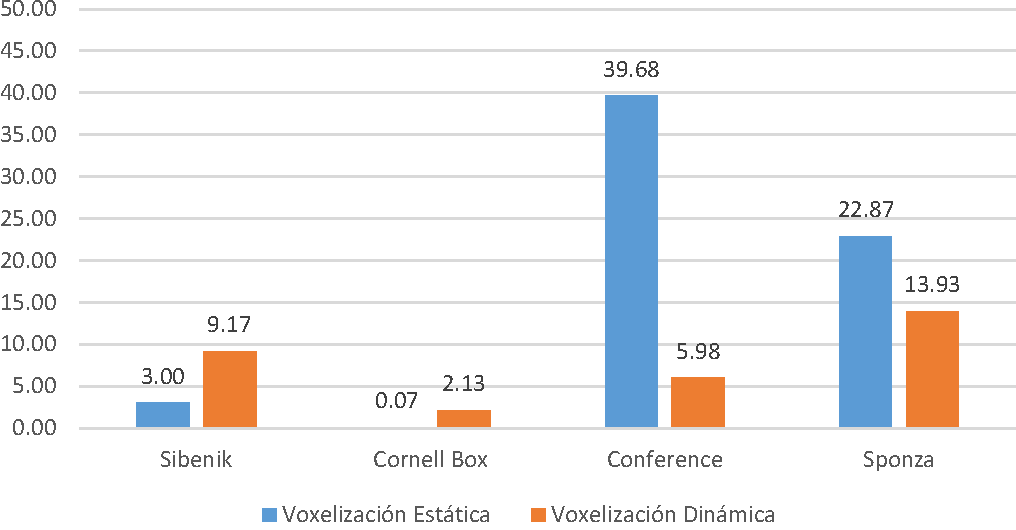
\includegraphics[width=\linewidth]{media/voxelzation_64_cropped.pdf}
		\caption*{Resolución de volúmenes: $64^3$}
	\end{subfigure}
	\begin{subfigure}{.49\textwidth}
		\centering
		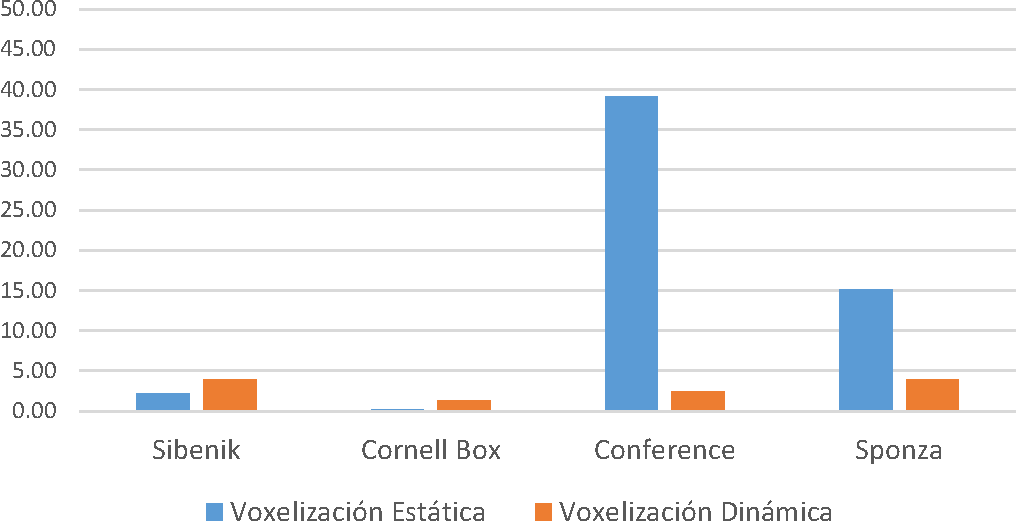
\includegraphics[width=\linewidth]{media/voxelzation_128_cropped.pdf}	
		\caption*{Resolución de volúmenes: $128^3$}
	\end{subfigure}
	\par\bigskip
	\begin{subfigure}{.49\textwidth}
		\centering
		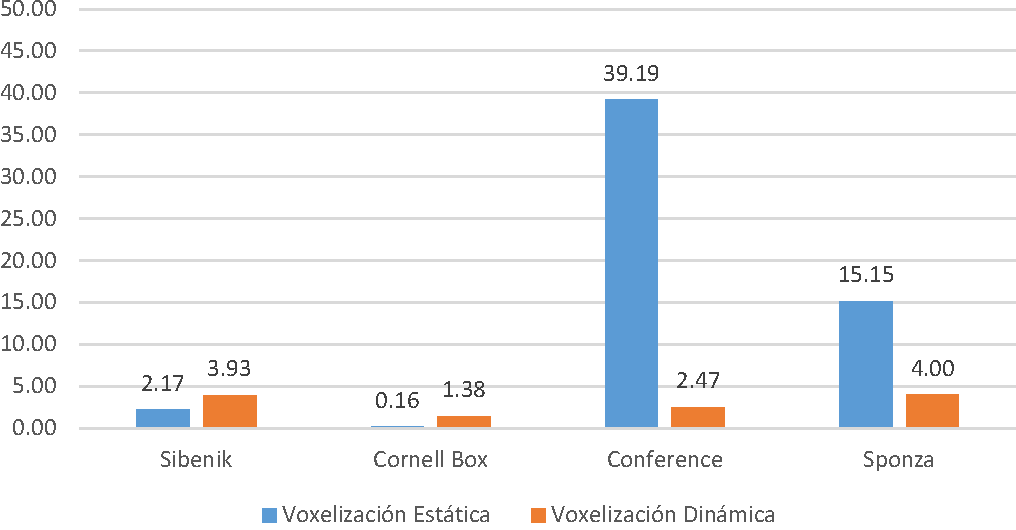
\includegraphics[width=\linewidth]{media/voxelzation_256_cropped.pdf}
		\caption*{Resolución de volúmenes: $256^3$}
	\end{subfigure}
	\begin{subfigure}{.49\textwidth}
		\centering
		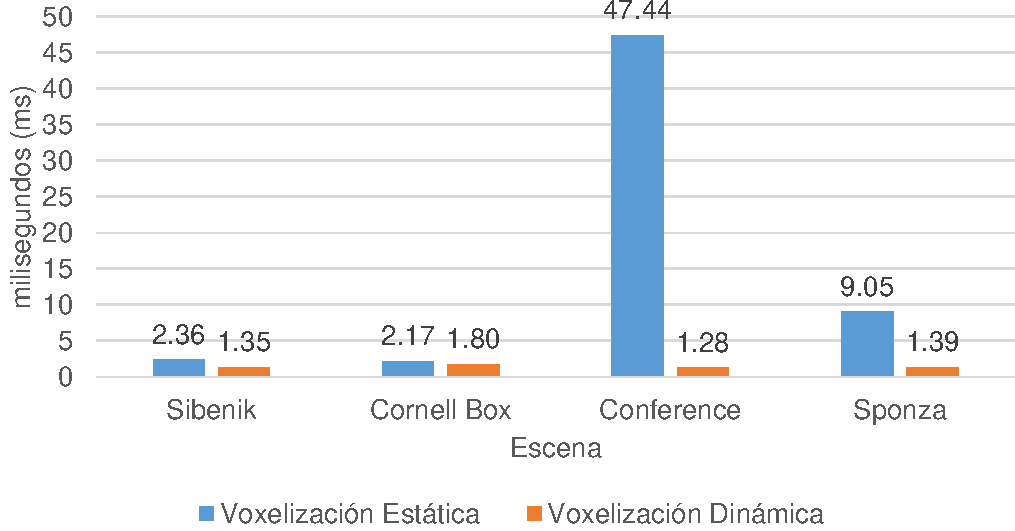
\includegraphics[width=\linewidth]{media/voxelzation_512_cropped.pdf}	
		\caption*{Resolución de volúmenes: $512^3$}
	\end{subfigure}
	\caption{Tiempos de voxelización dinámica y estática de escenas completas con distintas resoluciones para la representación en vóxeles.}
	\label{fig:voxelization_times}
\end{figure}

\subsubsection{Vacuidad y Velocidad de Trazado para la Iluminación Global de Vóxeles.}

En escenas donde existen muchos espacios vacíos el trazado de rayos suele tardar un poco más que en escenas densas de objetos. Esto se debe a que mientras la representación en vóxeles sea vacía en la posición que describe la apertura, dirección y punto de origen del cono, este cono debe seguir expandiéndose. A consecuencia mientras más espacios vacíos la representación en vóxeles tenga, más distancia tiene que recorrer cada cono aumentando la cantidad de operaciones de lectura sobre la representación en vóxeles.

Este problema se puede observar en la figura \ref{fig:gi_voxel_time} para las escenas Sponza y Cornell Box. La escena Cornell Box es en gran parte vacua con solo dos cuboides internos. La escena Sponza es densa en su interior por tanto la falta de objetos no es el principal problema. El problema de la Sponza reside en que la escena es larga y alta pero no ancha. Durante la voxelización cada triángulo se proyecta de forma ortogonal sobre cada eje para maximizar la voxelización, este frustum de proyección es cuadrado. Para las dimensiones de esta escena siempre quedara una cantidad considerable de vóxeles vacíos fuera de la geometría principal de la escena. 

% Una forma de evitar estos problemas en escenas como Sponza es comprobar que la posicion de trazado actual esta fuera de los limites de la escena, sin embargo esto puede ocasionar problemas visuales dependiendo de la apertura del cono en ese punto, para limitar correctamente el punto de trazado con respecto a los limites de la escena es necesario calcular la interseccion del cono contra el volumen delimitante.

\begin{figure}[h]
	\centering
	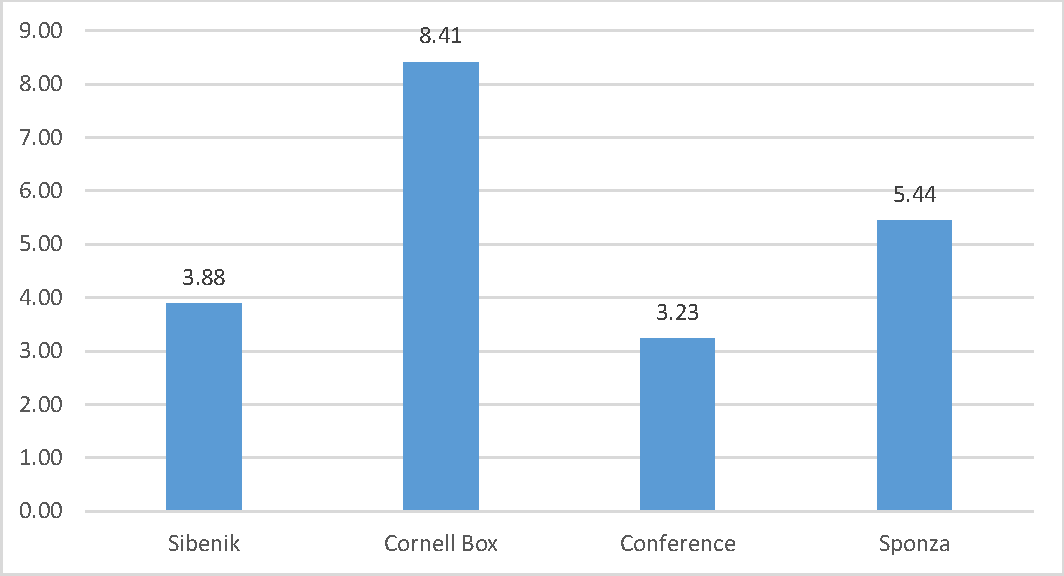
\includegraphics[width=0.85\linewidth]{media/voxel_gi_time_cropped.pdf}
	\caption{Tiempos de cálculo de iluminación global sobre la representación en vóxeles para todas las escenas completas.}
	\label{fig:gi_voxel_time}
\end{figure}

\subsection{Trazado de Sombras y Volumen de Visibilidad}

La aplicación provee sombras suaves para luces direccionales, puntuales y focales utilizando trazado de conos. Si no se sombrea la representación en vóxeles la imagen resultante es incorrecta a pesar de definir los contornos de sombreado. La razón es que el trazado de conos para la iluminación indirecta consideraría estos vóxeles como iluminados en vez de ocluidos por sombras. Nuestra implementación provee un método de inclusión de sombras suaves durante el sombreado de vóxeles. En esta sección se examina el rendimiento de las distintas opciones para el trazado de sombras que provee nuestra implementación excepto mapeado de sombras disponible solo para luces direccionales.

Estas pruebas utilizan todas las escenas completas. La configuración del escenario comprende solo una luz puntual con trazado de sombras habilitado. La cámara en escena es colocada de tal forma que todos los fragmentos visibles formen parte del trazado de conos. Con respecto a la configuración de la aplicación, se activo el modo de actualizacion forzosa para simular luces en constante movimiento y se desactivo la illuminacion global de voxeles.

Para estas pruebas se consideran distintas opciones en la aplicacion relevantes al trazado de sombras. Estas opciones comprenden: trazado de sombras durante el sombreado de vóxeles, trazado de sombras con trazado de conos y vóxeles o muestreo del volumen de visibilidad y distintas aperturas del cono utilizado para trazado de sombras.



\subsection{Apertura del Cono Especular}
